% Created 2022-11-03 jue 13:49
% Intended LaTeX compiler: pdflatex
\documentclass[12pt]{article}
\usepackage[latin1]{inputenc}
\usepackage[T1]{fontenc}
\usepackage{graphicx}
\usepackage{grffile}
\usepackage{longtable}
\usepackage{wrapfig}
\usepackage{rotating}
\usepackage[normalem]{ulem}
\usepackage{amsmath}
\usepackage{textcomp}
\usepackage{amssymb}
\usepackage{capt-of}
\usepackage{hyperref}
\usepackage[spanish]{babel}
\usepackage{graphicx,geometry}
\geometry{ a4paper, left=1in, right=1in, top=1in, bottom=1in }
\renewcommand\familydefault{\sfdefault}
\usepackage{sectsty}
\sectionfont{\normalfont\Large }
\subsectionfont{\normalfont\normalsize}
\usepackage{tabularx}
\usepackage{listings}
\lstdefinestyle{mystyle}{
numbers=left,
showspaces=false,
frame=leftline,
showspaces=false,
showstringspaces=false,
showtabs=false,
numberstyle=\tiny,
}
\lstset{
style=mystyle,
literate={�}{{\'a}}1
{�}{{\'e}}1
{�}{{\'{\i}}}1
{�}{{\'o}}1
{�}{{\'u}}1
{�}{{\'A}}1
{�}{{\'E}}1
{�}{{\'I}}1
{�}{{\'O}}1
{�}{{\'U}}1
{�}{{\"u}}1
{�}{{\"U}}1
{�}{{\~n}}1
{�}{{\~N}}1
{�}{{?``}}1
{�}{{!``}}1
}
\makeatletter
\usepackage{fancyhdr}
\pagestyle{fancy}
\usepackage{mdframed}
\BeforeBeginEnvironment{minted}{\begin{mdframed}}
\AfterEndEnvironment{minted}{\end{mdframed}}
\author{Luis Eduardo Galindo Amaya (1274895)}
\date{03-11-2022}
\title{C�lculo de C cuantil}
\hypersetup{
 pdfauthor={Luis Eduardo Galindo Amaya (1274895)},
 pdftitle={C�lculo de C cuantil},
 pdfkeywords={},
 pdfsubject={},
 pdfcreator={Emacs 26.3 (Org mode 9.1.9)}, 
 pdflang={Spanish}}
\begin{document}


\newcommand{\docente}{Olivia Mendoza Duarte}
\newcommand{\asignatura}{Estad�stica Avanzada}
\newcommand{\semestre}{2022-2}

\newcommand{\miportada}[1]{
	\begin{titlepage}
		\vspace*{0.75in}
		\begin{flushleft}
			\sffamily
			\large #1       \\
			\Huge
            \@title         \\
			\hrulefill
			\vspace{0.25in} \\
			\Large \@author \\
			%% \vspace*{\fill}
            %% 
\includegraphics[width=\textwidth]{../includes/filler.png} \\
			\vspace*{\fill}
			\large
			\begin{tabular}{|l|l|}
              \hline
			  Asignatura & \asignatura \\
			  Docente    & \docente    \\
			  Fecha      & \@date      \\
              \hline
			\end{tabular}
		\end{flushleft}
	\end{titlepage}
}

\miportada{ notas }

\fancyhf{}
\lhead{ \asignatura }
\rhead{ \semestre }
\rfoot{P�gina \thepage}

\setlength\parindent{0pt}   % eliminar el intentado
\setlength{\parskip}{1.2em}

\maketitle
\end{center}

\section*{Ejercicio de calificaciones}
\label{sec:org1cfa6f3}
\subsection*{Calcule}
\label{sec:org870fdbe}
El cuartil 0.65 y El cuatil 0.42

\begin{description}
\item[{1}] Ordenar el arreglo de forma asenente
\item[{2}] \(c' = 0,65 + 20 = 13\) y \(c' = 0,42 + 20 = 8,4\)
\item[{3}] \(Ccuantil = \frac{x'_{13} + x'_{14}}{2} = \frac{84+84}{2} = 84\) y \(Ccuantil = \left| 84 \right| + 1 = c9 = 69\)
\end{description}

\subsection*{Solucion}
\label{sec:orga9eabf4}
\begin{itemize}
\item a) El 65\% de las calificaciones est� por debajo del 84.
\item b) El 42\% de las calificaciones est� por debajo del 69.
\end{itemize}

\subsection*{Programa}
\label{sec:orgd73b8c5}
\begin{verbatim}

## cuartil de interes
cuartil_de_interes <- 0.42

## datos
x <- c(
  45, 69, 79, 83, 38, 27, 98, 100, 84, 79, 67, 84, 92, 35, 56, 69,
  47, 95, 100, 86
)

## ordenar los datos
x <- sort(x)

## cuartil
c <- cuartil_de_interes * length(x)

# check fractional part
Ccuartil <- if (c %% 1 == 0) {
  ## formula para enteros
  (x[c] + x[c + 1]) / 2
} else {
  ## formula para flotantes
  x[floor(c) + 1]
}

Ccuartil
\end{verbatim}

\pagebreak

\section*{Informacion del Dataset}
\label{sec:orgb3d700b}
\subsection*{Real estate valuation data\footnote{\url{https://archive.ics.uci.edu/ml/datasets/Real+estate+valuation+data+set}}}
\label{sec:org991cff0}
\begin{itemize}
\item 1. id
\item 2. the transaction date (for example, 2013.250=2013 March, 2013.500=2013 June, etc.)
\item 3. the house age (unit: year)
\item 4. the distance to the nearest MRT station (unit: meter)
\item 5. the number of convenience stores in the living circle on foot (integer)
\item 6. the geographic coordinate, latitude. (unit: degree)
\item 7. the geographic coordinate, longitude. (unit: degree)
\item 8. house price of unit area
\end{itemize}

\section*{Resultados}
\label{sec:orga51ac58}
Se utiliaron los datos de la columnas 3 (the house age (a�os) y 4 (distancia a una estacion MRT)
de todas las casas en el dataset se determino que la mitad de ellas: tienen menos de \textbf{16 a�os} de 
que fueron contruidas y estan a menos de 492.23 metros de distancia de una  estacion de MRT\footnote{Metro.}.

\section*{C�digo}
\label{sec:org0e50de0}
\lstinputlisting{./cuartiles.R}

\section*{Capturas}
\label{sec:org4a70b30}
\begin{figure}[htbp]
\centering
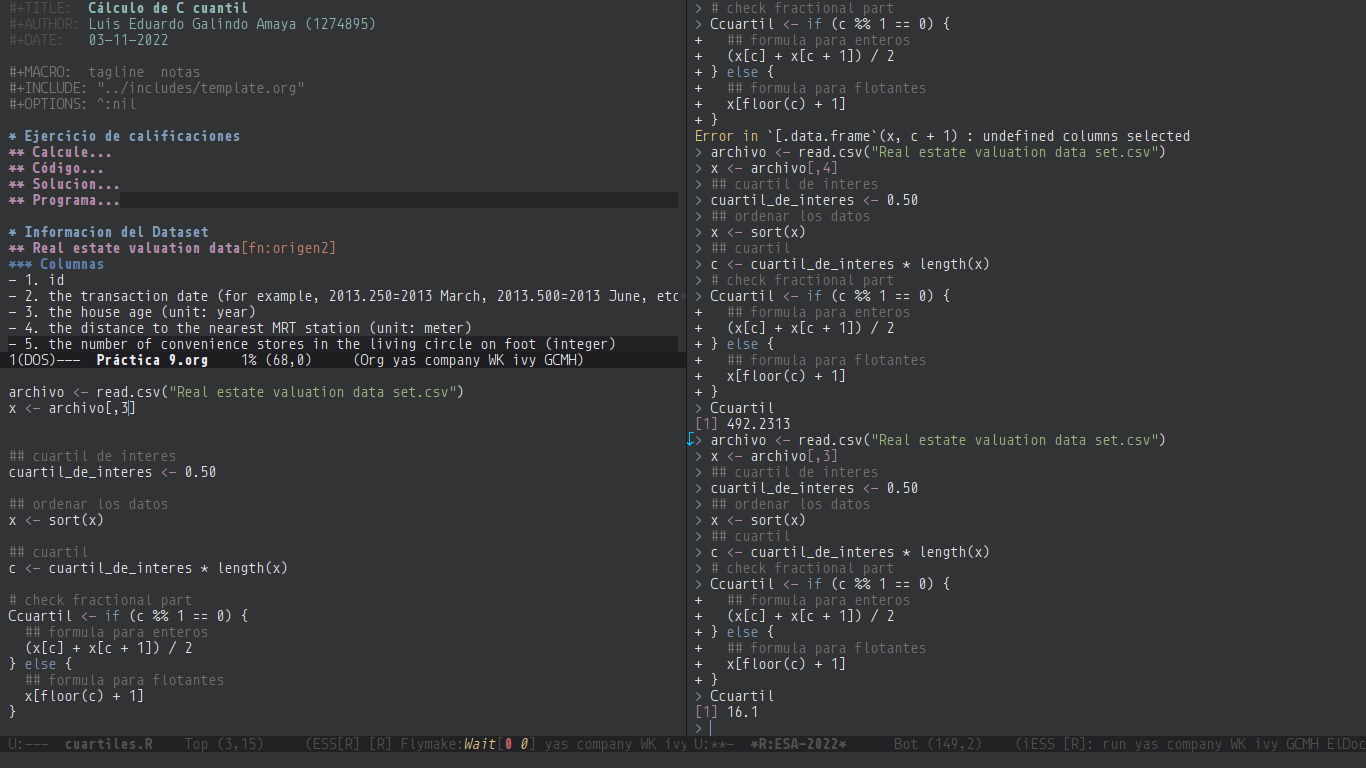
\includegraphics[width=10cm]{img/1.png}
\caption{Programa mostrando el cuatil .50 mostrando la antig�edad de las casas.}
\end{figure}

\begin{figure}[htbp]
\centering
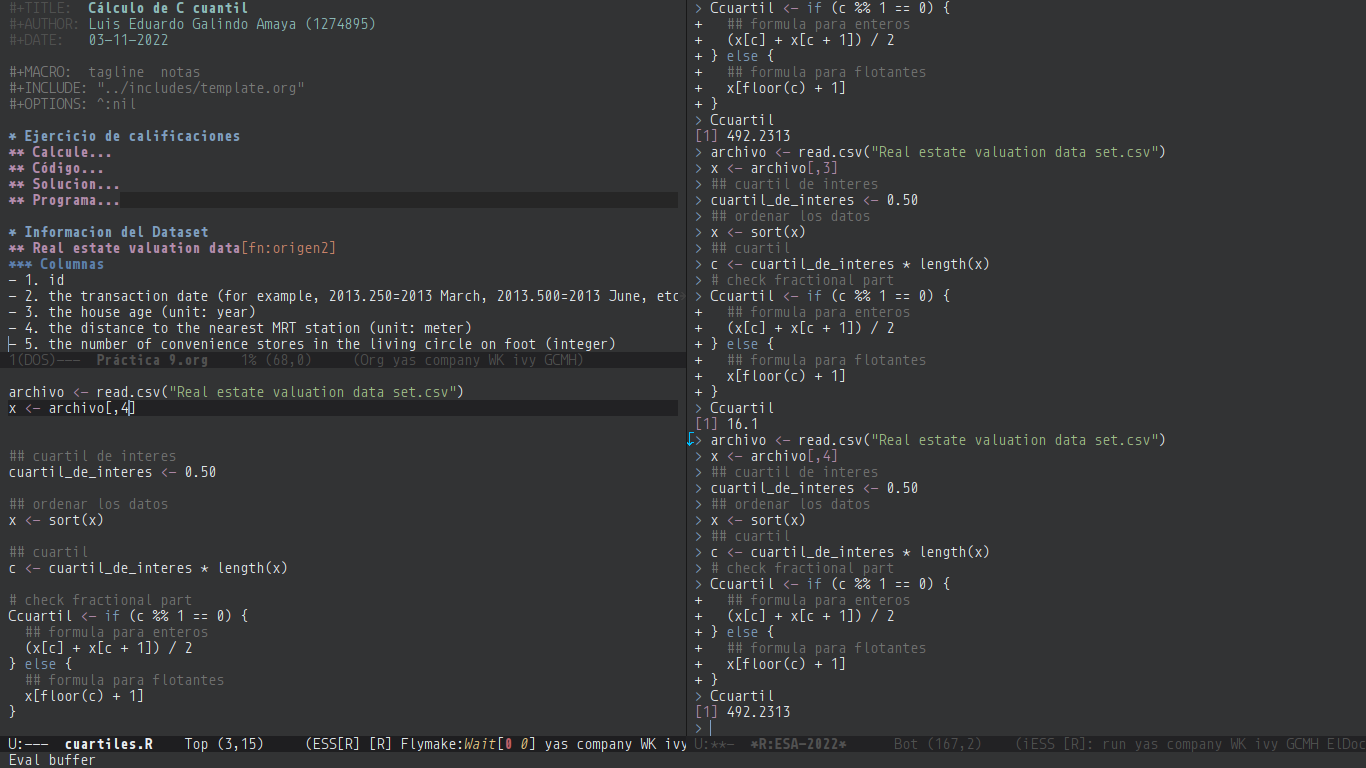
\includegraphics[width=10cm]{img/2.png}
\caption{Programa mostrando la distancia promedio a la estacion MRT m�s cercana.}
\end{figure}
\end{document}
